\documentclass[a4paper,11pt]{article}
\usepackage[utf8]{inputenc}
\usepackage[T1]{fontenc}
\usepackage{amsmath}
\usepackage{mathtools}
\usepackage{amsfonts}
\usepackage{amssymb}
\usepackage{graphicx}
\usepackage{multicol}
\usepackage{array}
\usepackage{float}
\usepackage{epstopdf}
\usepackage{caption}
\usepackage{subcaption}
\usepackage{gensymb}
\usepackage[bottom]{footmisc}
\usepackage{appendix}
\usepackage{pdfpages}
\usepackage{todonotes}
\usepackage{mathpazo}
\usepackage{titleps}
\usepackage{color}
\usepackage{xcolor}
\usepackage{colortbl}
\usepackage{siunitx}
\usepackage{pdflscape}
\usepackage{cancel}

\usepackage[skins]{tcolorbox}
\usepackage{sectsty}
\usepackage[arrowmos]{circuitikz}
\usepackage{pgfplots}
\usepackage{blindtext}
\usepackage[inner=2cm,outer=2cm,top=2.5cm,bottom=2.5cm]{geometry}
\usepackage{todonotes}
\usepackage{hyperref}
\usepackage{url}
\usepackage{adjustbox}
\usepackage{tabularx}
\usepackage{booktabs}
\usepackage{fancybox}
\usepackage[tikz]{bclogo}



%For code insertion
%listing
\usepackage{listings}
\usepackage{xcolor}
\definecolor{codegreen}{rgb}{0,0.6,0}
\definecolor{codegray}{rgb}{0.5,0.5,0.5}
\definecolor{codepurple}{rgb}{0.58,0,0.82}
\definecolor{backcolour}{rgb}{0.98,0.98,0.98}
\lstdefinestyle{mystyle}{
    backgroundcolor=\color{backcolour},
    commentstyle=\color{codegreen},
    keywordstyle=\color{blue},
    numberstyle=\tiny\color{codegray},
    stringstyle=\color{codepurple},
    basicstyle=\ttfamily\footnotesize,
    breakatwhitespace=false,
    breaklines=true,
    captionpos=b,
    keepspaces=true,
    numbers=left,
    numbersep=5pt,
    showspaces=false,
    showstringspaces=false,
    showtabs=false,
    tabsize=2
}
\lstset{style=mystyle}



\graphicspath{{figures/}}
\sectionfont{\large}
\subsectionfont{\normalsize}



%%%%%%%%%%%%%%%%%%%
% HANDS-ON NUMBER
\newcommand\handsOnN{FPGA}
% WEEK NUMBER
\newcommand\weekN{8}
%%%%%%%%%%%%%%%%%%%

\newpagestyle{main}{
	\sethead[LELEC2102: Hands-on \handsOnN][][Week \weekN]{LELEC2102: Hands-on \handsOnN}{}{Week \weekN}
	\headrule
    \setfoot[][\thepage][]{}{\thepage}{}
}

\newcommand{\horrule}[1]{\rule{\linewidth}{#1}} % Create horizontal rule command with 1 argument of height
%\setlength {\marginparwidth }{2cm}
%%%%%%%%%%%%%%%%%%%%%%%%%%%%%%%%%%%%%%%%%%%%%%%%%%%%%%%%%%%%%%%%%%%%%%%%%%%%

\begin{document}
\renewcommand{\figurename}{Fig.}

\renewcommand{\thepage}{\arabic{page}}
\setcounter{page}{1}
\pagestyle{main}
\newpage \clearpage

\begin{center}
\begin{LARGE}
LELEC2103: Optimization
\end{LARGE}
\vspace{0.3cm}
%\textit{TA 1, TA 2}
\end{center}

\section*{Introduction}

In this Hands-On, you will be introduced to the basics of audio acquisition in an embedded context. This Hands-On is building up on the skills you developed during the H2a. Therefore, make sure you master the concepts, tools \textit{and} practical skills mentioned in that Hands-On. Moreover, make sure you have carefully read and understood the \texttt{Guide - how to use the boards.pdf} in the \texttt{Technical ressources} folder on Moodle. As for the H2a, we will provide you with a functional baseline code to start with for this Hands-On. Then, you will be guided step by step to develop the key skills needed for this part of the project.

\begin{bclogo}[couleur = gray!20, arrondi = 0.2, logo=\bcinfo]{Explanation of the hands-on boxes}
In this note, there are a few boxes presenting additional information:
\begin{itemize}
    \item \bcinfo will provide you some more detailed explanations.
    \item \bcattention will explain typical mistakes that might lead to errors or a non functional system.
    \item \bcquestion will provide you with additional questions or experiments that will improve your understanding of the system. We advise you to leave them for the end of the hands-on as they are not critical.
\end{itemize}
\end{bclogo}

\section*{Objectives}

\begin{itemize}
    \item Discover the Nucleo MCU board and its programming tools ;
    \item Learn the basics of bare metal embedded programming, General-Purpose Inputs-Outputs (GPIOs), interrupts and timers ;
    \item Understand qualitatively and measure quantitatively how the embedded software program impacts the MCU power consumption ;
    \item Learn how to debug an embedded program by logging/tracing and using a physical debugger.
\end{itemize}

%\section*{Material}

\begin{comment}[couleur = gray!20, arrondi = 0.2, logo=\bcinfo]{}
\vspace{0.2cm}
\end{comment}
For this hands-on session, you will need:
\begin{itemize}
    \item The latest version of STM32 Cube IDE installed on your host system (for further information, see INSTALL.md on the GitHub of the course) ;
    \item The Nucleo MCU board with its sensing and power-management board ;
    \item A USB cable to connect your computer to the Nucleo.
\end{itemize}
%\vspace{0.01cm}

\section{Accelerating the detection of the preamble}
In the previous Hands-On, our demodulation chain required a component called the \textit{preamble detector} that actively seeks the preamble sequence located at the beginning of a packet by looking at the energy of each sample and accumulating it over time. When the accumulated value exceeded a threshold, the preamble was considered present and a given amount of samples were forwarded to the synchronization stage. This system allows to avoid unnecessary heavy computations as well as real-time operation. There are two drawbacks to this process. First, the theshold is not updated and increasing the gain of the RF front-end will increase the noise power, possibly going above the set threshold. Second, this preamble detection scheme requires a lot of computation, calculating and accumulating the energy of each sample. As it operates continuously, it is best to move its functionality from software towards a specialized piece of hardware in order to improve its \textbf{energy efficiency and processing speed}. If we decide at one point to increase the packet rate of the overall transmission chain, this solution is more robust regarding packet misses. It is also further motivated by the fact that this block occurs at the very beginning of the processing chain, just after the low-pass filter we designed in the previous section. We will also change the behavior of the block by calculating the threshold based on the noise power and a given factor. The accelerated block will therefore be called the packet presence detector (PPD). However, we only want to accelerate the energy detection step but still receive all samples in GNU Radio to be able to monitor the channel if needed. Therefore, the PPD will add a flag at the start of a packet when it has been detected. This flag corresponds to the value \texttt{0x7FF} which can not be reached by the LMS7002M chip.


\subsection{Design overview}
We implemented for you a packet presence detection module in SystemVerilog HDL\footnote{Although uncommon, it is possible to mix multiple HDL languages in a single design. For instance, the majority of the LimeSDR-Mini system is written in VHDL, but for your convenience we have written the PPD in SystemVerilog.}. First, open the Quartus project, \texttt{LimeSDR-Mini\_lms7\_lelec210x/LimeSDR-Mini\_lms7\_lelec210x.qpf}. If a message asking you for overwriting the database is printed, click "yes". You can then open the PPD design file located in\\ \texttt{LimeSDR-Mini\_lms7\_lelec210x/ip/packet\_presence\_detection/packet\_presence\_detection.sv}\\ and containing the following interfaces:
\begin{itemize}
    \item A clock and reset interface.
    \item A sink (input) streaming interface with data and valid signals.
    \item A source (output) streaming interface with data and valid signals.
    \item A custom static interface for configuration signals.
\end{itemize}
The PPD follows the low-pass filter in the receiver chain, as you have seen in previous hands-on. The filter, implemented using a FIR, is already included in the hardware design provided to you. Indeed, as a FIR is composed of multiply-and-accumulate operations, it can be easily accelerated in hardware. The  PPD module is integrated as a custom IP inside the same subsystem as the FIR, it therefore shares the same streaming interfaces\footnote{See pp 40-52 of \texttt{mnl\_avalon\_spec.pdf} on Moodle for details.}: the data bus is 24-bit wide with the MSBs and LSBs containing the samples of the I and Q channels respectively. In addition a valid signal is associated with the streaming data to indicate whether the data bus contains information of interest, or not. With the preamble detector, the goal is to produce an output valid signal that indicates if the complex magnitude of the data has reached a threshold.

\subsection{Packet presence detector schematic}
In Figure \ref{fig:pd_schematic} below you can find a schematic of the different modules that compose the preamble detector. As a reminder, the objective of this block is to add a flag at the start of a packet when a sufficient energy has been detected in the signal. It functions as follows:
\begin{enumerate}
    \item \textbf{Complex to magnitude: } The IQ samples are processed by a \textit{complex to magnitude} block which outputs the magnitude of the complex IQ vector.
    To do so, we calculate the magnitude as the square root of $I^2+Q^2$. As square-root function are difficult to implement in hardware logic, we are thus going to use a very simple and accurate algorithm. The estimate for the first quadrant of the trigonometric circle is drawn on Figure \ref{fig:cmplx2mag}. The mathematical formula is provided to you in Equation \ref{eq:1norm}\footnote{Further information can be found online: \url{https://en.wikipedia.org/wiki/Alpha_max_plus_beta_min_algorithm} and \url{http://dspguru.com/dsp/tricks/magnitude-estimator/}.}.

    \begin{equation}
        |z| = \frac{min(|I|,|Q|)}{4} + max(|I|,|Q|)
        \label{eq:1norm}
    \end{equation}
    
    \begin{figure}[h]
        \centering
        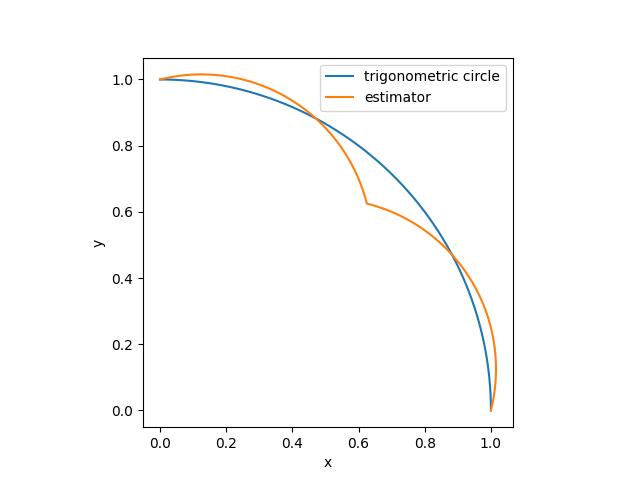
\includegraphics[width=0.45\linewidth]{figures/trigo.png}
        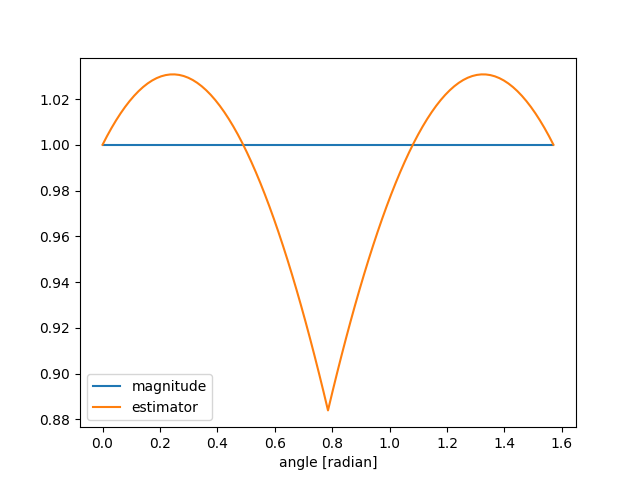
\includegraphics[width=0.45\linewidth]{figures/angle.png}
        \caption{Complex Magnitude Estimator output in x-y coordinates (left) or polar coordinates (right) for input points of the trigonometric circle.}
        \label{fig:cmplx2mag}
    \end{figure}

    \item \textbf{Dual running sum: } The estimated complex magnitude is then averaged over multiple samples by two moving average filter of different length in series, a short-term sum and long-term one. They are implemented by forwarding input samples in  memory-based \textit{delay lines}, developped by Altera. 

    \begin{align}
            y[n] = \sum_{k=0}^{N-1}\left|x[n-k]\right|
    \end{align}

    At each clock cycle an accumulator adds and substracts the first and last magnitudes stored in the delay line to its content. This structure is more efficient than the general FIR because we know each tap is equal to one, we therefore only need two adders. 

    \begin{align}
            y[n+1] = y[n] + \left|x[n]\right| - \left|x[n-N+1]\right|
    \end{align}

    The two moving average filters have two different functions. The first one, the short-term sum, receives the sample magnitudes first and its delayed output value are then forwarded to the long-term sum. It uses a longer delay line and is used to evaluate the noise power. 

    \begin{figure}[h]
        \centering
        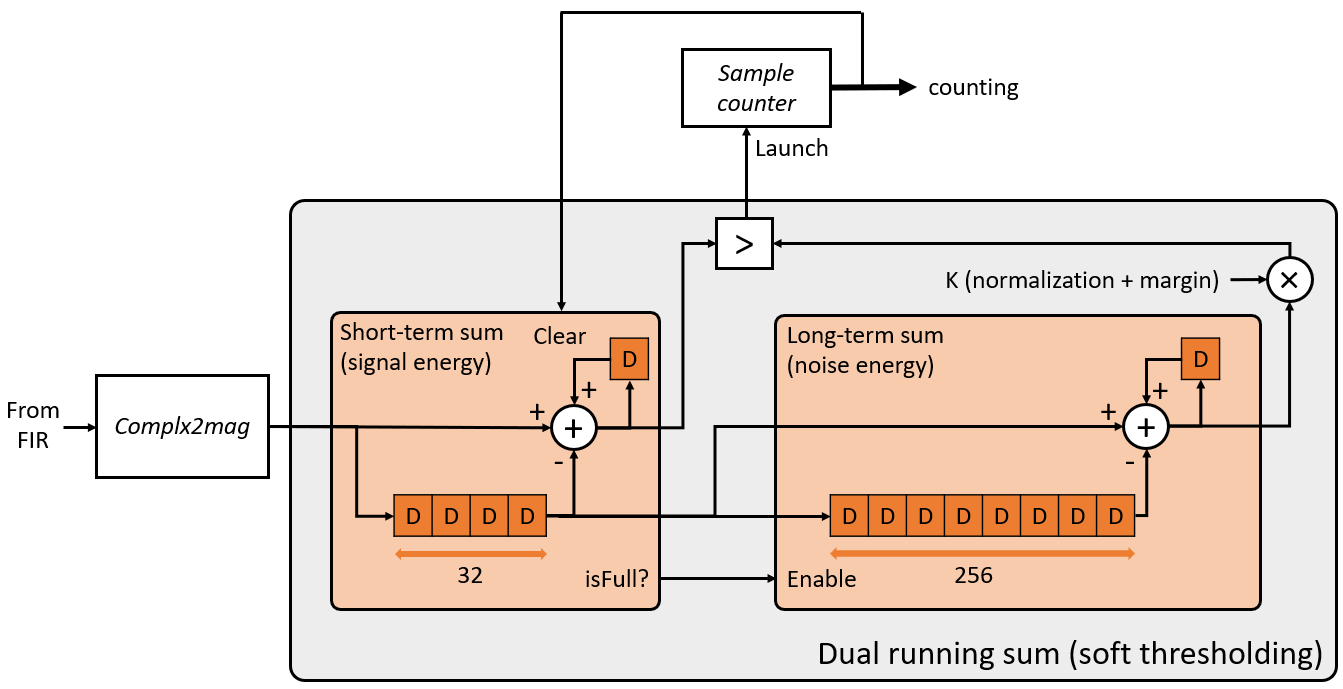
\includegraphics[width=\linewidth]{figures/dual_running_sum_block.png}
        \caption{Architecture of the dual running sum}
        \label{fig:dual_runnign_sum}
    \end{figure}
    
    The overall architecture of the dual running sum is shown in Fig. \ref{fig:dual_runnign_sum}. When packet samples arrive, possibly with  higher energy than the noise, they first enter the first delay line. Its accumulator value therefore increases and might at one point exceed the accumulator value of the second line, which contains only noise sample. At this point, a packet is considered present and a launch signal is triggered. 

    To be noted, when a packet is detected and the counter (next block) is enabled, we clear the short-term sum and disable the long-term one, to avoid any retriggering or corruption of our noise evaluation by packet samples.


    \item \textbf{Counter :} This block receives the launch signal of the previous one. This counter block is used to count the samples when the threshold has been reached and avoid triggering a start flag multiple times inside a single packet. A \texttt{launch} signal starts the counter, it stops only after reaching its maximum value. During the sequence a \texttt{running} signal indicates the state of the counter. This signal is used to clear the short-term sum of the dual running sum.

    \item \textbf{Flag addition :} A multiplexer is used at the end to set a sample to a flag, here $I=$\texttt{0x7FF} and $Q=$\texttt{0x7FF}  when the launch signal is triggered.

\end{enumerate}


\begin{figure}[h]
    \centering
    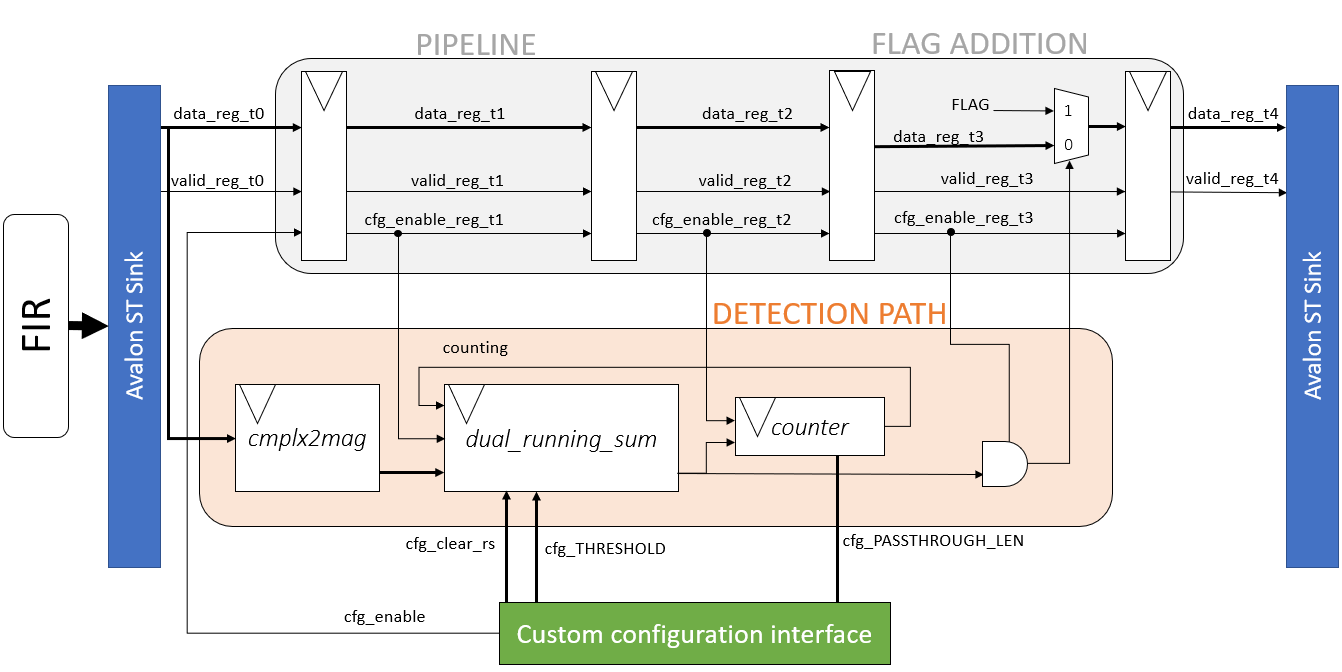
\includegraphics[width=\linewidth]{figures/packet_presence_detection.png}
    \caption{Hardware packet presence detector schematic}
    \label{fig:pd_schematic}
\end{figure}

In order to reduce the length of the critical path between registers, we use a paradigm called \textit{pipelining}. In short, we divide the operations of the PPD into several stages with similar length. As the critical path in this configuration is much shorter, it allows to operate the circuit at a higher frequency. In return, the additional registers add area and energy consumption to the design. It also requires to forward control signals in the pipeline and it can add complexity (see \textit{Control Path} in Figure \ref{fig:pd_schematic}). You will learn the concept of pipelining in details when studying the \textit{pipelined processor} in the course of \texttt{LELEC2531}.

Try to understand the SystemVerilog implementation of those blocks with respect to their theoretical behavior. Pay particular attention to the bus width of intermediate signals, they are computed in order to systematically avoid any overflow of intermediate values!


\subsection{Modification and simulation of the PPD}


We will first ask you to make some modifications to the dual running sum, more specifically to the comparison between the short- and long-term sum results. In order to make it adaptative from GNU Radio, we will use the \texttt{cfg\_THRESHOLD} signal of the packet presence detection module to multiply the result of the long-term sum before comparing it to the short-term sum result. This allows to be more selective regarding the signal-to-noise ratio required to detect the packet. Increasing its value will limit the risk of false alarm due to noise but make your system less sensitive. In short, with this parameter set to 10, the PPD would require a signal magnitude 10 times higher than the noise one to trigger a detection. However, we should also normalize the short-term and long-term result with respect to the delay line length, the second one being here eight times longer than the first. Overall, we ask you to implement the multiplication shown in Figure \ref{fig:dual_runnign_sum}. In the SystemVerilog code, go to the line 199. We ask you to implement both the normalization, i.e. division by eight, and the multiplication operation on the same line. Note that the \texttt{cfg\_THRESHOLD} signal is connected to the \texttt{K} input of the dual running sum module.


\begin{bclogo}[couleur = gray!20, arrondi = 0.2, logo=\bcquestion]{Division by eight}
    \begin{itemize}
        \item Performing multiplications and divisions is much more complex than simple additions. However, when performing operations with values that are power-of-two, things always seem easier. What would be an efficient way to perform the division by eight?
        \item The order in which the two operations are performed, here the multiplication by K and division by eight would normally have no importance. Is it the case here? Which operation should be performed first and why?
    \end{itemize}
\end{bclogo}

Once you have implemented this function, we should now test the PPD. We have developped a testbench for you, and we will use ModelSim to verify the PPD behavior before deploying it into the complete system. A few python scripts located at \texttt{ip/packet\_presence\_detection/testbench/python} allow you to generate input vectors for the PPD and compare the testbench output with an expected result obtained with python:

\begin{enumerate}
    \item \texttt{1\_input\_gen.py} : generates input vectors and export them as input vector of the PPD HDL implementation.
    
    \item To generate the testbench, we will use the \textit{Platform Designer}. It allows the interconnection of multiple blocks of a digital design with a more intuitive user interface. Open the \textit{Platform Design} using the shortcut highlighted in Figure \ref{fig:quartus_platform_designer}. Open the \texttt{packet\_presence\_detection\_tb\_gen}, and go in \textit{Generate} in the upper left corner, then \textit{Generate Testbench System}. Change the path to \texttt{LimeSDR-Mini\_lms7\_lelec210x/ip/packet\_presence\_detection/} and click on \textit{Generate}. To execute the testbench, open ModelSim and change the working directory to\\ \texttt{ip/packet\_presence\_detection/testbench}. Then run \texttt{do run\_sim.tcl} in order to compile and launch the simulation.

\begin{figure}[H]
    \centering
    
\includegraphics[scale=0.7]{figures/quartus_toolbar.PNG}
    \caption{Toolbar of Quartus. The Platform Designer shortcut is highlighted in yellow.}
    \label{fig:quartus_platform_designer}
\end{figure}

    \item \texttt{2\_compare} : when the SystemVerilog testbench has been executed, compares the input data samples to the output of the PPD, plotting them. If it works as expected, the only difference should be the addition of the flag.
\end{enumerate}

Once you have analysed the results, we will propagate the changes you made to the complete system that will be flashed on the FPGA. Remember we only modified the IP, we now need to propagate those changes to the actual design. In the \textit{Platform Designer}, open the \texttt{lms\_dsp.qsys} design. Nothing has to be done except clicking \textit{"Generate HDL ..."} on the bottom right of the window and update the path to
\texttt{LimeSDR-Mini\_lms7\_lelec210x/lms\_dsp/} if it is not made automatically. Then press on \textit{"Generate"}. The changes you made locally to the PPD have now been propagated. In the Platform Designer, you can quickly observe the structure of the \textit{lms\_dsp} block, with the FIR, the packet presence detection and the different Avalon Streaming Interface.

You can now compile your design and observe the resource and timing report. Be careful when launching a compilation in Quartus, a window may ask you to update the project revision. Answer \textit{"NO"}.

\begin{bclogo}[couleur = gray!20, arrondi = 0.2, logo=\bcattention]{MAX 10 Device Support might not be installed}
    The support for the FPGA device we use might not be installed in the Quartus you have, which will lead to errors in the compilation. The installation instructions are provided in the wiki of the course.

\end{bclogo}

\subsection{Timing and ressource analysis}

As you have seen in course, an important aspect of digital design is to ensure that your design meet both the resource and timing requirements. Indeed, long combinatorial logic path can lead to setup or hold constraints violations. Now that the design has been compiled, you can check the compilation report using the shortcut highlighted in Figure \ref{fig:compilation_report_button}. 

\begin{figure}[h]
    \centering
    
\includegraphics[width=\linewidth]{figures/Compilation_report_button.PNG}
    \caption{Toolbar of Quartus. The Compilation Report shortcut is highlighted in red.}
    \label{fig:compilation_report_button}
\end{figure}


In the \textit{"Flow Summary"} tab, the resource utilisation is reported. Observe for instance the number of embedded multipliers that are employed. Moreover, in the \textit{"Analysis \& Synthesis/Timing Analyzer"} tab, you can see the results for the different corners, constraints violations being highlighted in red. Try to identify the faulty clock involved. In the different summary proposed, you can right click on a clock and select \textit{"Report Timing... (In Timing Analyzer UI)"}. In the opened window, just press \textit{"Report Timing"} at the bottom. Those steps are depicted in Figure \ref{fig:report_timing_analyzer}. You can now analyze the most critical path implying the selected clock, as well as the logic cells involved. Try to link the critical path to the RTL design. It should involve a signal starting in the dual running sum module. An easy fix is here to add a register in the path to break in two. This will delay the launch signal by one clock cycle, which is not problematic. 

\begin{figure}[h]
    \centering
    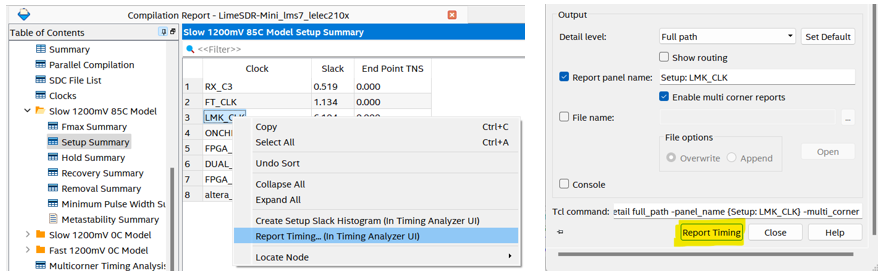
\includegraphics[width=\linewidth]{figures/Report_Timing_Analyzer.png}
    \caption{Steps to analyze the most critical path on a given clock.}
    \label{fig:report_timing_analyzer}
\end{figure}

Moreover, we prevented \textbf{register retiming} which allows the synthesis tool to balance the combinatorial logic across registers when it does not affect the system behaviour. This helps on meeting the timing requirements by offloading parts of long combinatorial path. To enable this setting, go in \textit{"Assignments/Settings/Compiler Settings"} on Quartus and uncheck the \textit{"Prevent register retiming"} box.

Before relaunching a compilation, ask for an assistant to check your modifications, to avoid wasting precious synthesis time. Done? Now relaunch a compilation and analyze the results. Again, if a window asks you to update the project revision, answer \textit{"NO"}. Is there still a timing constraint violation? Can you still link the most critical path to the HDL design?

To analyse the ressource used by the design, you can look at the \textit{Project Navigator} tab in \textit{Hierarchy}. More than navigating through the design, you can also look at the ressource used by each module. Analyse the resource usage of the PPD, more specifically the memory bits and the DSP.
\begin{comment}
\subsection{From Euclidean norm to Absolute-value norm}

In order to meet the timing requirements, another solution is to use a less complex estimation of the IQ samples magnitude. We are thus going to use a very simple and accurate algorithm that does not have the burden of implementing the complex logic of \textit{integer multiplication}. The estimate for the first quadrant of the trigonometric circle is drawn on Figure \ref{fig:cmplx2mag}. We ask you to implement it in System Verilog, the mathematical formula being provided to you in Equation \ref{eq:1norm}\footnote{Further information can be found online: \url{https://en.wikipedia.org/wiki/Alpha_max_plus_beta_min_algorithm} and \url{http://dspguru.com/dsp/tricks/magnitude-estimator/}.}. Your modification of the \texttt{cmplx2mag} module must be done in the \texttt{USER CODE} parts, which goes from line 45 to 52 and on line 210. As we were performing two multiplications and one addition in the previous algorithm ($I^2+Q^2$), the data bus at the output of the \textit{cmplx2mag} module was specified as twice the input data bit width (due to multiplication) plus one (due to the addition). This is specified on line 210, do not forget to adapt it for the new algorithm. In the next step, you are going to make a behavioral simulation of you implementation to validate it.

\begin{equation}
    |z| = \frac{min(|I|,|Q|)}{4} + max(|I|,|Q|)
    \label{eq:1norm}
\end{equation}

\begin{figure}[h]
    \centering
    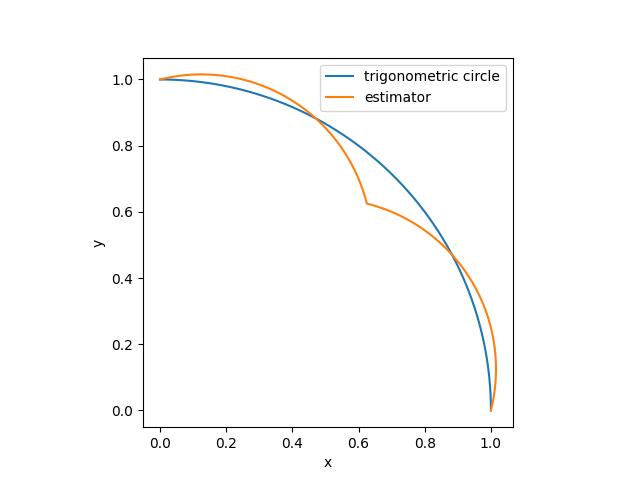
\includegraphics[width=0.45\linewidth]{figures/trigo.png}
    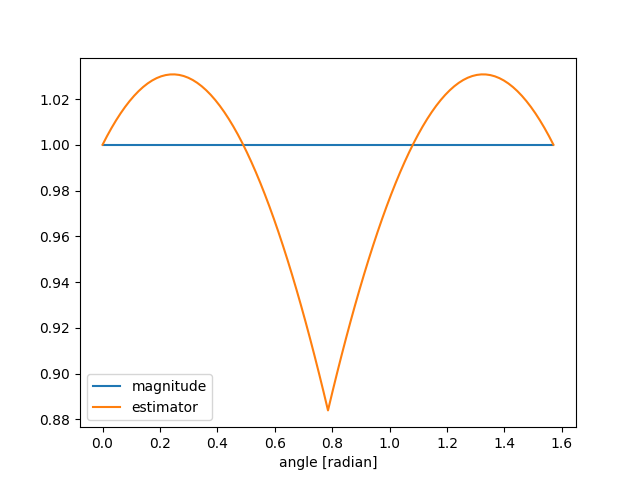
\includegraphics[width=0.45\linewidth]{figures/angle.png}
    \caption{Complex Magnitude Estimator output in x-y coordinates (left) or polar coordinates (right) for input points of the trigonometric circle.}
    \label{fig:cmplx2mag}
\end{figure}


Now that you have a functional design for the preamble detector with the Absolute-value norm, we can perform a synthesis of the complete design. Do not forget to propagate your change by regenerating the HDL via the Platform Designer. Observe the resource usage and the timing report, is there still a timing constraint violation?

\end{comment}

\section{Overview of communication chain}
In this section, the different steps involved in the communication chain are presented.

\subsection{Transmitted signal}
The idea behind 2-FSK or 2-CPFSK modulations is to send waveforms at different frequencies based on the input bit sequence. Usually, the bit sequence is first converted into a symbol sequence $\mathbf{I}$. In a binary case, the symbol mapping can be the following: a symbol $I=1$ is sent when the bit to send is a $1$ whereas the symbol $I=-1$ is associated to the bit $0$. In this case, the two reference waveforms in baseband are:
\begin{equation*}
    e_I(t)\:=\:\exp{\left(j 2\pi I \Delta_f t \right)}\:=\:\begin{cases}
    e_{s_1}(t)\:=\:\exp{\left(j 2\pi \Delta_f t \right)}\:\:\:\text{if}\:\: I=1,\\
    e_{s_0}(t)\:=\:\exp{\left(-j 2\pi \Delta_f t \right)}\:\:\:\text{if}\:\: I=-1,
    \end{cases}
\end{equation*}
with $\Delta_f$ the frequency deviation (in hertz). This is only what is sent over one symbol period $T$. Following the lecture developments, the baseband representation of a whole 2-CPFSK signal is given by
\begin{equation*}
    x(t)\:=\:e^{j\phi(t)} \qquad \text{with} \qquad \phi(t)\:=\:\:2\pi \Delta_f \int_{-\infty}^t \sum_{k=-\infty}^{\infty}I[k]\:g(\tau-kT) \text{d}\tau,
\end{equation*}
where $\phi(t)$ is the phase, $T$ is the symbol period (in second) and $I[k]$ is the k-th sent symbol. Moreover, $g(t)$ is a rectangular pulse shaping filter defined only on a symbol period, i.e.,
\begin{equation*}
    g(t)\:=\:\begin{cases} 1 \qquad \text{for} \: 0 \leq t \leq T\\
    0 \qquad \text{otherwise.}
    \end{cases}
\end{equation*}
The use of $g(t)$ shifted by some symbol periods in the summation enables to represent continuously the symbol sequence, whereas the integration over $\tau$ ensures continuous phase.

\paragraph{Packet structure} In practice, for the LELEC2102-3 project, the bit sequence is not sent continuously. Instead, they are grouped in several packets, each of them having the structure presented in \autoref{tab:packet_struc}. This packet structure comes from the specifications of the radio (RF transceiver) used in the project (S2-LP device from STMicroelectronics, see \href{https://www.st.com/resource/en/datasheet/s2-lp.pdf}{\textcolor{blue}{[S2-LP datasheet]}}).
\begin{table}[H]
\centering
\caption{Packet structure.}
\begin{tabular}{|c|c|c|c|}
\hline
\rowcolor[HTML]{C0C0C0}
Preamble   & Sync word  & Payload       &  CRC             \\ \hline
4 bytes    & 4 bytes    & 0:65535 bytes & 1 byte           \\
\py{0xAAAAAAAA} & \py{0x3E2A54B7} & ...           & Based on payload \\ \hline
\end{tabular}
\label{tab:packet_struc}
\end{table}
The different parts of the packets are motivated by their respective roles:
\begin{itemize}
    \item The preamble is a repeating sequence that enables to easily identify the beginning of a packet. Usually, the repeating bit sequence is made of "$01$" or "$10$".
\item The sync word is a chosen sequence that is known by the receiver. It is useful for synchronization purposes and can be chosen. In the basic version of the project, it is arbitrarily set to \py{0x3E2A54B7}.
    \item The payload contains the message bits. Its length can vary but will be fixed to a given value to ensure packets of same length.
    \item CRC (cyclic redundancy check): is used in practice to detect transmission error and drop packets containing errors. It is not implemented in the simulation framework but it will be used in the practical chain (see next hands-on).
\end{itemize}


\subsection{Channel model}
For this project, we neglect multipath propagation such that the channel is considered to be flat fading. In this case, using the channel equivalent baseband representation, the received signal $y(t)$ is modeled by
\begin{equation*}
    y(t) = a\: e^{j\phi_0}\: e^{j2\pi \Delta f_c t} \:x(t-\tau) + w(t),
\end{equation*}
where $a$ is the attenuation, $\phi_0$ is the phase shift and $\Delta f_c$ is the carrier frequency offset. Furthermore, $\tau$ depicts the delay, such that $\tau=kT+\tau_d$ with $k$ an integer and $\tau_d$ a delay between 0 and $T$. Finally, $w(t)$ is an additive white Gaussian noise (AWGN).



\subsection{Reception chain}
Based on the channel model and the packet structure, the reception chain of \autoref{fig:comm_chain} has been defined by the teaching team. At the input of the receiver, one has access to the complex baseband signal $y(t)$ sampled at a given sampling frequency whereas, at the output of the reception chain, the payload bits are recovered.

\begin{figure}[H]
    \centering
    
\includegraphics[width=\textwidth]{figures/comm_chain.pdf}
    \caption{Reception chain.}
    \label{fig:comm_chain}
\end{figure}

Currently, we will focus on this chain in simulation but starting from next hands-on, the blocks highlighted in orange in \autoref{fig:comm_chain} will be implemented in GnuRadio whereas the red blocks will execute in hardware. This chain contains the following blocks:

\paragraph{Low-pass filter}
This filter limits the noise bandwidth at the input of the reception chain.

\paragraph{Preamble detection}
The goal of the preamble detection is to determine the start of packets: when it detects a packet (based on its preamble energy for example), this packet is forwarded to the next steps of the chain and is demodulated. When no packets are detected, nothing is demodulated and computational resource is spared.

\paragraph{Synchronization}
This block is responsible for the CFO (carrier frequency offset) and STO (symbol timing offset) synchronizations. In other words, it estimates and corrects the frequency offset $\Delta f_c$ as well as the fractional delay $\tau_d$. However, no phase estimation ($\phi_0$) is performed.


\paragraph{Demodulation}
The demodulator recovers the symbol sequence based on the CPFSK modulated signal and converts these symbols back to bits. Its output is therefore a bit sequence, containing the preamble, sync word, payload and CRC bits. Since the phase shift $\phi_0$ has not been corrected, non-coherent demodulation is used.

\paragraph{Packet parser}
Finally, the packet parser is responsible for determining the beginning of the payload bits in the bit sequence coming from the demodulator. As such, it recovers the frame delay $kT$. The CRC is also checked to determine if all bits have been demodulated properly.

\subsection{Simulation framework}
The provided simulation framework contains four files:
\begin{itemize}
    \item \textbf{sim.py}: this is the body of the simulation framework. It modulates the sent packets, applies the channel and uses the synchronization and demodulation functions implemented by \texttt{Chain} subclasses. It provides several performance metrics as outputs. Normally, you should not modify anything in this file, except the plots at the end if you want to customize them and the simulated chain at the very bottom. You can also add an automatic save of the simulation data to post-process it later on. Nevertheless, you are highly encouraged to skim through the file and the comments to understand the different steps involved.
    \item \textbf{chain.py}: this contains the \texttt{Chain} with most of the modulation parameters and the prototypes of the modulation, demodulation and synchronization functions. You can change the modulation parameters in this file if you want to study their effects but you will implement the functions in subclasses, e.g., \texttt{BasicChain}.
    \item \textbf{test.py}: the purpose of this file is to help you to implement the demodulation and CFO estimation functions. Indeed, it contains a simplified version of the communication chain, useful for debugging your implementation.
\end{itemize}

In order to launch the simulation, you only have to execute the \textbf{sim.py} file as it includes and calls the two other files. Try to run the simulation. You should observe a bit error rate (BER) of 0.5 since the demodulation is not implemented.

In the next sections, we will investigate step by step the different blocks of the simulation framework.

\section{FSK modulation and demodulation}
We first consider the modulation and demodulation, leaving aside any synchronization issue.

\subsection{Modulation}
The simulation framework models the baseband signal $x(t)$ sampled at a given symbol period $T$. Moreover, an oversampling factor $R_{\text{TX}}$ is applied, meaning that samples of $x(t) $ are available every $T/R_{\text{TX}}$. In other words, $R_{\text{TX}}$ samples are available during the symbol period $T$ of one CPFSK symbol. Hence, the sampled baseband signal is defined by

\begin{equation*}
    x[m] \:=\:x\left(m\frac{T}{R_{\text{TX}}}\right)\:=\:\exp \left(j\pi \frac{h}{T} \int_{-\infty}^{\frac{mT}{R_{\text{TX}}}} \sum_{k=-\infty}^{\infty}I[k]\:g(\tau-kT) \text{d}\tau \right),
\end{equation*}
where $h=2 \Delta_f T$ is the modulation index.
Assuming a symbol mapping such as the bit $0$ (resp. bit $1$) corresponds to the symbol $-1$ (resp. symbol $1$), the associated Python code to generate $x[m]$ from an input bit sequence is given in \autoref{fig:code_mod}. It is not a direct application of the mathematics presented above but instead an iterative generation of the CPFSK waveform. Indeed, in the for loop, the phase continuity is ensured simply by storing in memory the ending phase of the previous symbol. The phase shift during one symbol is given by $\pm h\pi$.

\begin{listing}[H]
\inputpython{modulate.py}
\caption{Python code for 2-CPFSK modulation.}
\label{fig:code_mod}
\end{listing}



As an example, the 2-CPFSK signal of the bit sequence "$0010110$" modulated with a bit rate $B$ of \SI{50}{\kilo\hertz}, a frequency deviation $\Delta_f=\frac{B}{4}$ and a TX oversampling factor $R_{\text{TX}}=4$ is given in \autoref{fig:2CPFSKbaseband}\footnote{You can generate figures similar to this one using the file \textbf{test.py}.}. You can also observe the continuous analog waveform $x(t)$ in light blue. Make sure you understand the different representations given in the figure (complex baseband representations). Determine the symbol period and, looking at the evolution of the phase, try to recover the sent bits.

\begin{figure}[h]
    \centering
    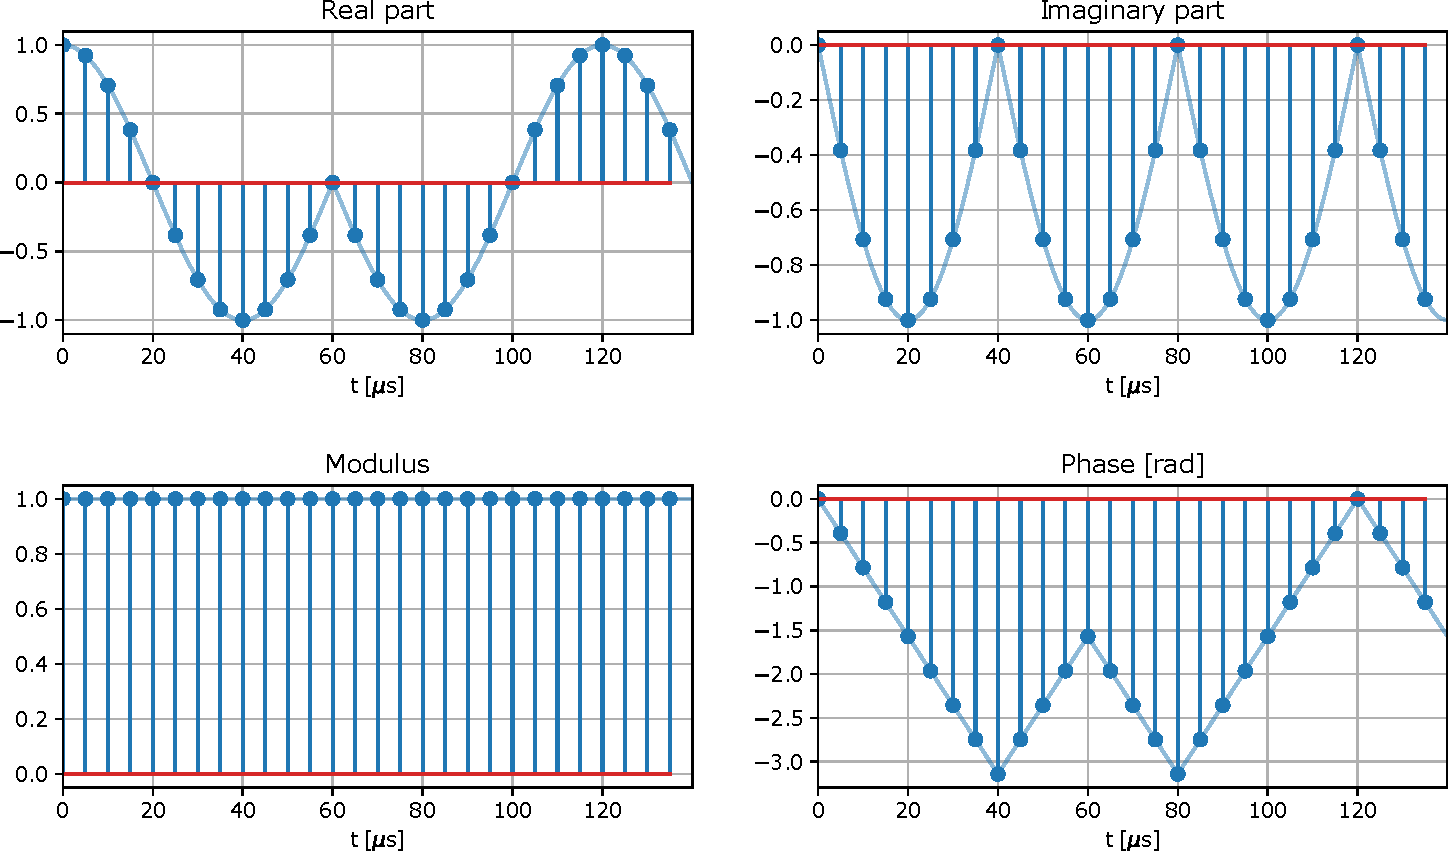
\includegraphics[width=0.8\textwidth]{figures/2-cpfsk-bis.pdf}
    \caption{Example of 2-CPFSK baseband signal of the bit sequence "$0010110$".}
    \label{fig:2CPFSKbaseband}
\end{figure}


\subsection{Demodulation}
Assuming perfect synchronization and no attenuation, the received signal is only impacted by the noise, such that
\begin{equation*}
    y(t)\:=\:x(t) + w(t).
\end{equation*}
Classically, for 2-FSK or 2-CPFSK modulations, one tends to demodulate the received signal by computing its correlations with the reference waveforms ($e_{s_1}(t)$ and $e_{s_0}(t)$ in baseband) \textbf{over each symbol period}:
\begin{equation*}
    r_1\:=\:\frac{1}{T}\int_0^T y(t)\:e_{s_1}^*(t) \:\text{d}t\qquad \text{and} \qquad r_0\:=\:\frac{1}{T}\int_0^T y(t)\:e_{s_0}^*(t) \:\text{d}t.
\end{equation*}

The \textbf{coherent detection} then compares the \textbf{real part} of $r_1$ and $r_0$ to select the largest as the most likely sent symbol. However, this assumes that the phase of the received signal is known, which is not the case here (as this would imply to add another synchronization block dedicated to the phase estimation).

In the case of \textbf{non-coherent detection}, the \textbf{modulus} of $r_1$ and $r_0$ is compared and the decision is taken as follows:
\begin{align*}
    &\hat{I}[k]=1 \: \:\:\:\:\:\:\:\text{if}\:\:\: |r_1| > |r_0|,\\
    &\hat{I}[k]=-1 \:\: \:\:\text{if}\:\:\: |r_1| < |r_0|.
\end{align*}

The decision is therefore taken symbol by symbol, considering the waveform $y(t)$ only during the symbol period $T$ of the symbol $I[k]$.

In practice, one does not have access to $y(t)$ but instead to $y[n]$, i.e., a sampled version with a symbol period $T$ and an oversampling factor $R_{\text{RX}}$ used at the receiver:
\begin{equation*}
    y[n]\:=\:y\left(\frac{nT}{R_{\text{RX}}}\right)\:=\:x\left(\frac{nT}{R_{\text{RX}}}\right)+w\left(\frac{nT}{R_{\text{RX}}}\right)\:=\: x[n] + w[n].
\end{equation*}
Therefore, the decision variables $r_1$ and $r_0$ for the symbol $I[k]$ are approximated by:
\begin{small}
\begin{equation*}
    r_1\:\approx\:\frac{1}{R_{\text{RX}}}\sum_{n=0}^{R_{\text{RX}}-1} y[kR_{\text{RX}}+n] \:\exp \left(-j2\pi \Delta_f \frac{nT}{R_{\text{RX}}}\right)\qquad \text{and} \qquad r_0\:\approx\:\frac{1}{R_{\text{RX}}}\sum_{n=0}^{R_{\text{RX}}-1} y[kR_{\text{RX}}+n] \:\exp \left(j2\pi \Delta_f \frac{nT}{R_{RX}}\right).
\end{equation*}
\end{small}

\begin{bclogo}[couleur = gray!20, arrondi = 0.2, logo=\bccrayon]{Implementation of demodulation}
Complete the \py{demodulate()} function in the file \textbf{chain.py} based on the development presented above (non-coherent detection) and the comments. Test your implementation using \textbf{test.py} and make sure the demodulated bits are the same as the sent ones (since there is no added noise).
\end{bclogo}

\subsection{BER-SNR curve}
Due to the noise on the received signal, the demodulation may suffer from errors. In the simulation, the noise is added on each sample by taking an independent realisation of a complex normal random variable with zero-mean $\mathcal{CN}(0,\sigma_w^2)$. The noise power in discrete time is given by the variance $\sigma_w^2$ of the complex normal random variable and can be linked to the signal-to-noise ratio (SNR), knowing that the sent waveforms are normalized (i.e., power of 1):
\begin{equation*}
    \text{SNR}\:=\:\frac{1}{\sigma_w^2}.
\end{equation*}

This SNR is therefore defined on each sample, meaning that a SNR of 0 dB implies that the instantaneous power of the signal is equal to the average power of the noise. This SNR is known in the simulation framework but in practice you may have to estimate it, see appendix \ref{appA}.




\paragraph{Bit error rate}
Often, the demodulation performances of a communication chain are determined by measuring the bit error rate (BER). It is defined as the probability of making a demodulation error on a bit. To compute it in simulation, many iterations are performed with thousands of bits sent and the error probability is simply obtained by counting the number of bits demodulated properly and the ones suffering from a demodulation error. Thus the simulation framework can directly output a simulated BER-SNR curve, for the range of SNRs specified in \textbf{chain.py}.

This simulated BER-SNR curve can then be compared to some theoretical curves, obtained thanks to mathematical developments based on the decision variable and the model of the noise (AWGN). For example, the bit error probability in the case of a BPSK transmission if given by
\begin{equation*}
    p_{e,\text{BPSK}}\:=\:\frac{1}{2} \text{erfc}\left(\sqrt{\text{SNR}_o}\right),
\end{equation*}
where $\text{SNR}_o$ is the SNR on the decision variable.

In the case of a FSK transmission with orthogonal signals, the bit error probability is
\begin{equation*}
    p_{e,\text{FSK}}\:=\:\frac{1}{2} \text{erfc}\left(\sqrt{\frac{\text{SNR}_o}{2}}\right).
\end{equation*}

Finally, when non-coherent (nc) detection is used with (CP)FSK orthogonal signals:
\begin{equation*}
    p_{e,\text{FSK nc}}\:=\:\frac{1}{2}e^{-\text{SNR}_o/2}.
\end{equation*}

The expressions of these theoretical curves enable you to compare your simulation results with the theory. However, the theoretical expressions involve the SNR on the decision variable, denoted $\text{SNR}_o$, and not directly the SNR defined previously, on each sample. The link between these two quantities is extracted from the definition of the decision variable. For example, the decision variable $r_1$ when the sent symbol $I[k]$ is a $1$ is (looking only over one symbol, assuming $k=0$ for simplicity):
\begin{small}
\begin{align*}
    r_1\: &= \:\frac{1}{R_{\text{RX}}}\sum_{n=0}^{R_{\text{RX}}-1} y[n] \:\exp \left(-j2\pi \Delta_f \frac{nT}{R_{\text{RX}}}\right)\\
    &=\:\frac{1}{R_{\text{RX}}}\sum_{n=0}^{R_{\text{RX}}-1} \left(\exp \left(j2\pi \Delta_f \frac{nT}{R_{\text{RX}}}\right)+w[n]\right) \:\exp \left(-j2\pi \Delta_f  \frac{nT}{R_{\text{RX}}}\right)\\
    &=\:1\:+\:\frac{1}{R_{\text{RX}}}\sum_{n=0}^{R_{\text{RX}}-1} \underbrace{w[n] \:\exp \left(-j2\pi \Delta_f \frac{nT}{R_{\text{RX}}}\right)}_{w'[n] \:\sim\: \mathcal{CN}(0,\sigma_w^2)}\:=\:1\:+\:\underbrace{\frac{1}{R_{\text{RX}}}\sum_{n=0}^{R_{\text{RX}}-1} w'[n]}_{\tilde{w}},
\end{align*}
\end{small}
because the exponential is just introducing a phase shift of the noise and thus does not change its variance. Since the $w'[n]$ are independent and identically distributed, the variable $\sum_{n=0}^{R_{\text{RX}}-1} w'[n]$ follows a distribution $\mathcal{CN}(0,R_{\text{RX}}\sigma_w^2)$ and $\tilde{w}\:\sim\:\mathcal{CN}(0,\frac{\sigma_w^2}{R_{\text{RX}}})$. The $\text{SNR}_o$ on the decision variable $r_1$ is therefore given by the ratio between the power of the useful signal ($=1$) and the power of the noise ($=\sigma_w^2/R_{\text{RX}}$):
\begin{equation*}
    \text{SNR}_{o}\:=\:\frac{R_{\text{RX}}}{\sigma_w^2}\:=\:R_{\text{RX}}\: \text{SNR}.
\end{equation*}
\textbf{This expression is only valid if the noise is white. If it has been filtered (i.e. the noise samples are correlated), it must be adapted.} Nevertheless,
this explains the SNR shift (in dB) that you can find in the simulation framework. Intuitively, it comes from the fact that $R_{\text{RX}}$ samples are aggregated together in the decision variable and add up coherently, whereas the $R_{\text{RX}}$ noise samples does not add coherently.

\begin{bclogo}[couleur = gray!20, arrondi = 0.2, logo=\bccrayon]{Simulation of BER-SNR curve}
You now have all the necessary explanations to understand the generation of BER-SNR curves by the simulation framework and compare them with the theory. In \textbf{chain.py}, make sure all the booleans bypassing the synchronization are set to \py{True}. Then, run the file and observe the generated BER-SNR curves. Do they stick to the theoretical curves?

Normally, your curve should have a trend similar to the theoretical curve, hinting that your demodulate function works properly. However, you can expect some differences but do not investigate them now. This will be part of the characterization report as well as of future improvements in the communication part of the project.

If needed, you can change the range of SNRs as well as the number of packets and the number of bits per packet in \textbf{chain.py}.
\end{bclogo}
\paragraph{Packet error rate (PER)} A packet is said to be erroneous if at least one bit of the packet is not demodulated properly. Following this definition, the probability of packet error $P_e$ is related to the bit error rate $p_e$ by
\begin{equation*}
    P_e\:=\:1- (1-p_e)^{N_b},
\end{equation*}
where $N_b$ is the number of bits in a packet and $(1-p_e)^{N_b}$ is the probability that all the bits of the packet are demodulated properly.
\begin{bclogo}[couleur = gray!20, arrondi = 0.2, logo=\bccrayon]{Simulation of PER-SNR curve}
In simulation, to obtain a meaningful PER curve, do not forget to increase the number of sent packets in \textbf{chain.py}.
\end{bclogo}



\section{Synchronization}
It is now time to tackle some synchronization issues, following the channel model and the reception chain presented in the first section. Most of it has already been implemented for you, based on the explanations given below.

\subsection{Preamble detection}
The preamble is made of a repeating sequence of bits "$10$". It enables to identify the start of a packet at the receiver, which is particularly useful for the practical chain. In order to study its performance in simulation, an extra sequence of pure noise is added in front of the packets to simulate the reception of noise when no packets are sent.

\paragraph{Energy detection} The algorithm chosen for the preamble detection is based on the received signal energy. The main idea is simply to take the modulus of the received samples and check that it is above a given threshold. In simulation, this threshold should be close to 1 since the received useful signal has an energy of 1. However, in practice, the received signal energy depends on the TX and RX gain, as well as the transmission distance. Therefore the threshold should be reduced to allow more flexibility in the communication range.

This energy detection can be performed sample by sample or using an averaging window of size $L$, as given in \autoref{fig:code_preb}. A preamble is detected if $\sum_{n=0}^{L-1}|y[n]| \: > \: \lambda$,
with $\lambda$ the energy threshold, and its position is then returned by the function.

\begin{listing}[H]
\begin{python}
from typing import Optional

import numpy as np

def preamble_detect(self, y: np.array) -> Optional[int]:
    """
    Detects the preamlbe in a given received signal.

    :param y: The received signal, (n * R,).
    :return: The index where the preamble starts,
        or None if not found.
    """
    L = 4*self.osr_rx
    y_abs = np.abs(y)

    for i in range(0, int(len(y)/L)):
        sum_abs = np.sum(y_abs[i*L:(i+1)*L])
        if sum_abs > (L-1): #fix threshold
            return i*L

    return None

\end{python}
\caption{Python code for preamble detection (from \textbf{chain.py}).}
\label{fig:code_preb}
\end{listing}

\paragraph{Metrics} The performance of the preamble detection algorithm can be evaluated with two metrics:
\begin{itemize}
    \item The percentage of false detection. A false detection occurs when the preamble detector triggers in the noise, when there is no packet to be found.
    \item The percentage of miss detection. A miss detection occurs when a preamble is not found or found too late (in the packet payload).
\end{itemize}

\begin{bclogo}[couleur = gray!20, arrondi = 0.2, logo=\bccrayon]{Simulation of preamble detection}
Set the bypassing boolean of the preamble detection to \py{False} in \textbf{chain.py}. Launch the simulation and observe the preamble detection metrics automatically displayed.
\end{bclogo}

\subsection{Frequency offset estimation}
The carrier frequency offset $\Delta f_c$ comes from a mismatch between the carrier frequency $f_c$ at the transmitter and the carrier frequency $f'_c$ used at the receiver: $\Delta f_c=f_c-f'_c$. This offset can also change over time due to temperature variations in the reference clocks generating the carrier frequencies at TX and RX. For the project, it has been decided to estimate the frequency offset for each received packet, assuming it is not varying during one packet duration (hypothesis verified in practice).

\paragraph{Moose algorithm} Based on repetition properties of a training sequence, the Moose algorithm can estimate the frequency offset from this sequence. Here, we use the repetition of "$10$" in the preamble, since the start of the preamble has already been roughly identified by the preamble detection block.

Disregarding other synchronization parameters except a frequency offset $\Delta f_c$, a received sequence containing a repetition of a block of size $N_t=N\cdot R_{\text{RX}}$ (with $N$ the number of CPFSK symbols) has the following property:

\begin{align*}
    y[n+N_t] \:&=\:e^{j2\pi \Delta f_c \frac{(n+N_t)T}{R_{\text{RX}}}} \:x\left(\frac{(n+N_t)T}{R_{\text{RX}}}\right) \:+\: w[n+N_t]\\
    &=\:e^{j2\pi \Delta f_c \frac{N_tT}{R_{\text{RX}}}} \underbrace{e^{j2\pi \Delta f_c \frac{nT}{R_{\text{RX}}}}\:x\left(\frac{nT}{R_{\text{RX}}}\right)}_{\approx y[n]} \:+\: w[n+N_t]\\
    &\approx \:e^{j2\pi \Delta f_c \frac{N_tT}{R_{\text{RX}}}}\: y[n].
\end{align*}
with the approximation coming from the noise realisations that are different on $y[n]$ and $y[n+N_t]$.

In order to estimate $\Delta f_c$ using this property, a modified least square problem can be formulated:
\begin{equation*}
    \hat{\alpha} = a \:e^{j2\pi \widehat{\Delta f_c} \frac{N_tT}{R_{\text{RX}}}} = \arg\min_{\alpha} \: \sum_{l=0}^{N_t-1} \left|y[l+N_t] - \alpha y[l]\right|^2.
\end{equation*}
The solution of this problem is given by
\begin{equation*}
    \hat{\alpha} =  \frac{\sum_{l=0}^{N_t-1} y[l+N_t]y^*[l]}{\sum_{l=0}^{N_t-1} |y[l]|^2},
\end{equation*}
and therefore the estimate of the frequency offset is obtained:
\begin{equation*}
     \widehat{\Delta f_c} = \frac{\arg\left\{\hat{\alpha}\right\}}{2 \pi \frac{N_tT}{R_{\text{RX}}}} = \frac{\arg\left\{\sum_{l=0}^{N_t-1} y[l+N_t]y^*[l]\right\}}{2 \pi \frac{N_tT}{R_{\text{RX}}}}.
\end{equation*}

Owing to the periodicity of the complex exponential, the Moose algorithm can estimate frequency offsets in the range $-\pi$ to $\pi$ for its argument, meaning that the range for $\widehat{\Delta f_c}$ is:
\begin{equation*}
    |\widehat{\Delta f_c}| \leq \frac{R_{\text{RX}}}{2N_tT}\:=\:\frac{B}{2N}.
\end{equation*}
In order to improve the estimation, a larger $N_t$ is preferable to increase noise averaging, but it reduces the range of non ambiguous frequency offset estimations. A solution to this issue can be based on multiple repetitions of short training sequences in the preamble.

\paragraph{Metric and correction}
The metric to monitor the accuracy of the frequency offset estimation is the root mean square error (RMSE), defined as
\begin{equation*}
    \text{RMSE}_{\Delta f_c}\:=\:T\sqrt{\left\langle\left(\widehat{\Delta f_c}-\Delta f_c\right)^2\right\rangle},
\end{equation*}
with $\left\langle ... \right\rangle$ denoting the mean over all iterations in the simulation, $\widehat{\Delta f_c}$ the estimated frequency offset and $\Delta f_c$ the real offset.

From the estimation of the frequency offset, the frequency offset correction is simply performed as follows:
\begin{equation*}
    \tilde{y}[n] = e^{-j2\pi \widehat{\Delta f_c} \frac{nT}{R_{\text{RX}}}}\:y[n].
\end{equation*}


\begin{bclogo}[couleur = gray!20, arrondi = 0.2, logo=\bccrayon]{Implementation of Moose algorithm}
Implement the Moose algorithm in the \py{cfo_estimation()} function in \textbf{chain.py}. The preamble has already been detected, such that the first samples of the input vector $y$ contains repeating sequence of modulated "$10$". Use blocks of 4 bits ($N=4$) and return $\widehat{\Delta f_c}$.

To test your implementation, first use \textbf{test.py} and make sure the estimated CFO corresponds to the applied one. You can then use the \textbf{chain.py} file, setting the CFO bypass boolean to \py{False}. Look at the RMSE, does it decrease with larger SNR?

By default, the CFOs applied in the simulation are random, in the range specified in \textbf{chain.py}. You can also decide to apply a constant frequency offset by giving a non-zero value to \py{cfo_val} in \textbf{chain.py} and removing \py{cfo_val = np.nan} in \textbf{chain.py}.
\end{bclogo}



\subsection{Symbol timing}
The symbol timing correction is performed after the correction of the frequency offset meaning that, ideally, the only remaining impairment (other than the timing error) is the noise. As already mentioned previously, the delay $\tau$ can be split in a delay multiple of the symbol period ($kT$ with $k$ an integer) and a fractional delay $\tau_d$ between 0 and $T$. The goal of the symbol timing block here is to correct the delay $\tau_d$ while the delay $kT$ is handled later by the frame estimation in the packet parser.

Since the received signal is oversampled by the factor $R_{\text{RX}}$, estimating $\tau_d$ resumes to choosing which sample (among $R_{\text{RX}}$ samples) defines the start of new CPFSK symbols. To do so, the multiple of $\frac{T}{R_{\text{RX}}}$
closest to $\tau_d$ is selected. This is illustrated in \autoref{fig:timing_ex} where $R_{\text{RX}}=4$ and the estimated symbol timing $\hat{\tau}_d$ is given by $\frac{dT}{R_{\text{RX}}}$.

\begin{figure}[H]
    \centering
    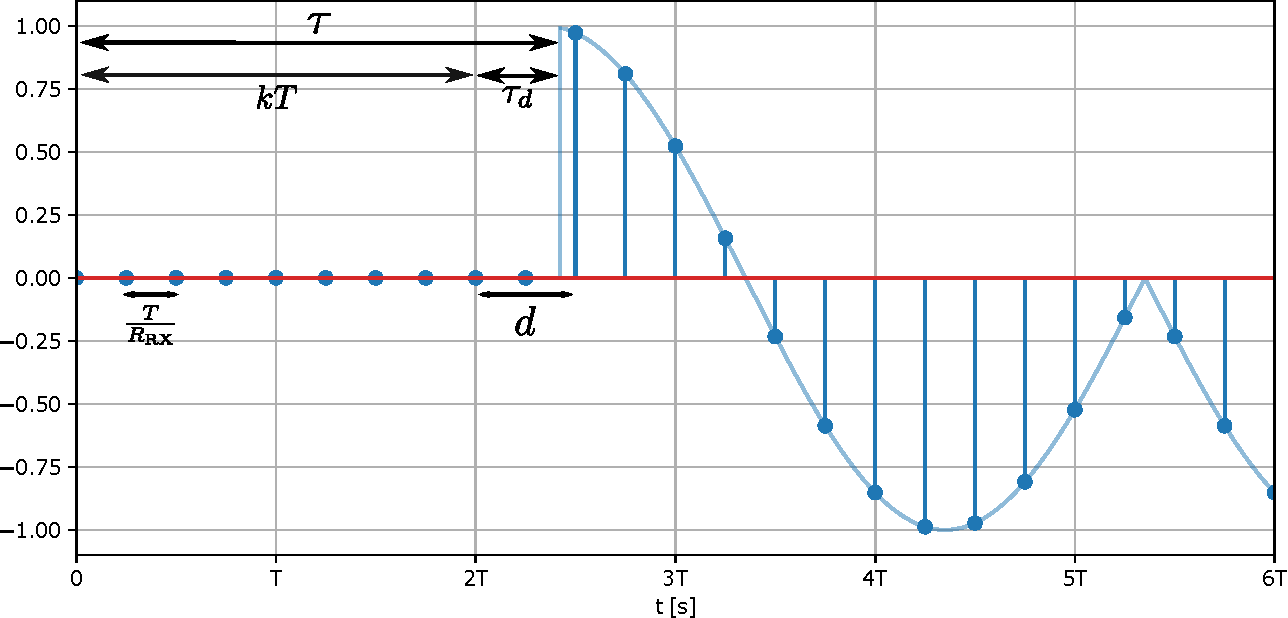
\includegraphics[width=0.82\textwidth]{figures/drawing_timing.pdf}
    \caption{Illustration of timing estimation (only real part of received signal is depicted).}
    \label{fig:timing_ex}
\end{figure}

It is possible to estimate the symbol timing by determining the instants where one observes a change in the derivative of the phase. This corresponds to a change in the sent waveform, that can happen only every multiple of the oversampling factor $R_{\text{RX}}$. As an example, \autoref{fig:phase_funct} gives the phase function and its derivatives corresponding to the sent bit sequence "$0010110$" with an oversampling factor $R_{\text{RX}}=32$. As expected, we identify peaks in the second derivative of the phase corresponding to the transition between symbols $1$ and $-1$ (and vice-versa).

With a delay $\tau_d$, all these peaks are not located in multiple of the symbol period but instead in $\tau_d+m T$ with $m\in \mathbb{Z}$. Then $\tau_d$ can be estimated using the function \py{sto_estimation()} in \textbf{chain.py}, as given in \autoref{fig:code_symb}.

\begin{figure}[H]
    \centering
    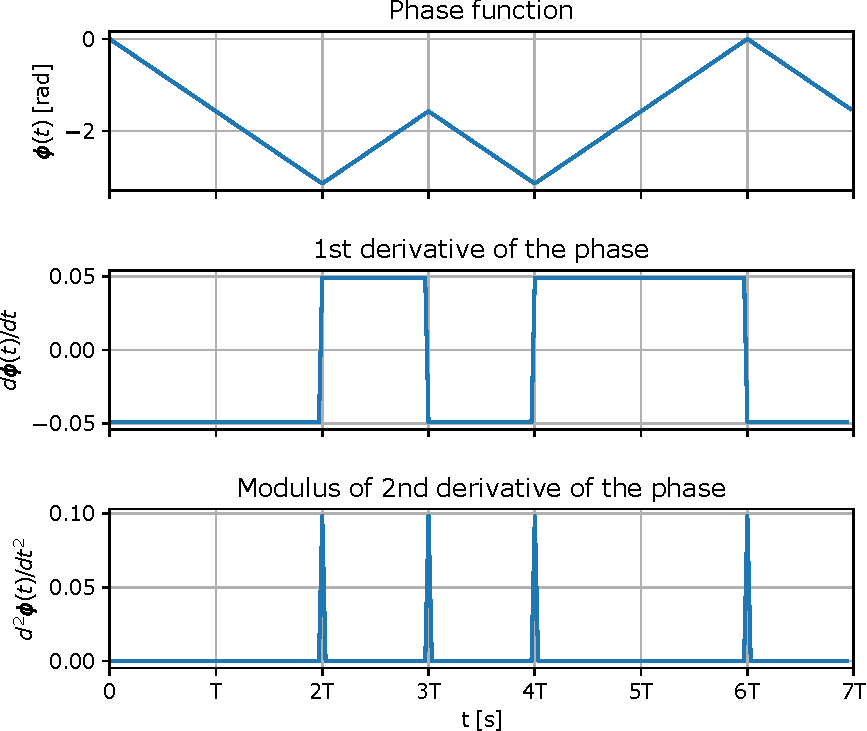
\includegraphics[scale=0.75]{figures/phase_function_bis.pdf}
    \caption{Example of a phase function and its derivatives for the bit sequence "0010110" with an oversampling factor $R_{RX}=32$.}
    \label{fig:phase_funct}
\end{figure}




\begin{listing}[H]
\begin{python}
import numpy as np

def sto_estimation(self, y):
    """
    Estimates symbol timing (fractional) based on phase shifts
    """

    R = self.osr_rx

    # Computation of derivatives of phase function
    phase_function = np.unwrap(np.angle(y))
    phase_derivative_1 = (phase_function[1:]-phase_function[:-1])
    phase_derivative_2 = np.abs(phase_derivative_1[1:]-phase_derivative_1[:-1])

    sum_der_saved = -np.inf
    save_i = 0
    for i in range(0,R):
        sum_der = np.sum(phase_derivative_2[i::R]) # Sum every R samples

        if sum_der > sum_der_saved:
            sum_der_saved = sum_der
            save_i = i

    return np.mod(save_i+1, R)

\end{python}
\caption{Python code for symbol timing estimation (from \textbf{chain.py}).}
\label{fig:code_symb}
\end{listing}


\subsection{Frame estimation}
Finally, only the frame estimation remains and is implemented in the packet parser. At this stage, bits have been demodulated and one is interested in knowing where the payload bits start.

Since the sent packets contain a sequence known by the receiver (the sync word sequence), the receiver can locate this sequence in the demodulated bits. Then the bits after this sequence will be the payload bits. This is achieved by performing a correlation between the demodulated bit sequence and the known sequence (\py{sync_word}, encoded in \textbf{chain.py}). This correlation is computed in \textbf{sim.py} by first converting the bit sequences into symbol sequences of $-1$ and $1$. The Python code is given in \autoref{fig:code_fr}.
\begin{listing}[H]
\begin{python}
import numpy as np

v = np.abs(np.correlate(bits_hat*2-1, np.array(chain.sync_word)*2-1, mode="full"))
start_frame = np.argmax(v)+1
bits_hat_pay = bits_hat[start_frame:start_frame+chain.payload_len]

\end{python}
\caption{Python code for frame estimation (from \textbf{sim.py}).}
\label{fig:code_fr}
\end{listing}

\paragraph{Metric} The accuracy of the total delay estimation can be evaluated with the RMSE:
\begin{equation*}
    \text{RMSE}_{\tau}\:=\:\frac{1}{T}\sqrt{\left\langle\left(\hat{\tau}-\tau\right)^2\right\rangle}\:=\:\frac{1}{T}\sqrt{\left\langle\left(\hat{d}\frac{T}{R_{\text{RX}}}+\hat{k}T-\tau\right)^2\right\rangle},
\end{equation*}
where $\hat{d}$ comes from the symbol timing estimation and $\hat{k}$ comes from the frame estimation.



\begin{bclogo}[couleur = gray!20, arrondi = 0.2, logo=\bccrayon]{Simulation of frame and symbol timing estimations}
Set the bypassing boolean of the symbol timing estimation to \py{False} in \textbf{chain.py}. Launch the simulation and observe the symbol timing RMSE automatically displayed. Does it decrease with increasing SNRs?

By default, the delays applied in the simulation are random, in the range specified by \py{sto_range} in \textbf{chain.py}. You can also decide to apply a constant timing offset by giving a non-zero value to \py{sto_val} in \textbf{chain.py} and removing \py{sto_val = np.nan} in \textbf{chain.py}.

\end{bclogo}

\section{Report R3a: simulation results}

We only ask a report at the end of the \textbf{next hand-on}. The report should contain a part dedicated to the simulation results, for which you may find the guidelines below.

This hands-on report (maximum 3 pages) should contain:
\begin{enumerate}
    \item A copy-paste of your implementations in the simulation framework:
    \begin{itemize}
        \item the \py{demodulate()} function in \textbf{chain.py};
        \item the \py{cfo_estimation()} function in \textbf{chain.py}.
    \end{itemize}
    \item Some BER-SNR simulation curves:
    \begin{itemize}
        \item a BER-SNR curve with perfect synchronization, showing the performance of your demodulation algorithm (all bypass booleans should be set to \py{True});
        \item a BER-SNR curve of the complete chain, involving all the synchronization blocks (all bypass booleans should be set to \py{False}).
    \end{itemize}
    Briefly comment the results by giving some hypotheses that could explain the differences between the curves with and without ideal synchronization. \textbf{For your simulation results to be meaningful, increase the number of sent packets and the number of bits per packet in \textbf{chain.py}}.
\item The simulated RMSE curve of the CFO estimation (with a random CFO in the range of \SI{1}{\kilo\hertz}, all bypass booleans set to \py{False}). Briefly explain the different trends observed in the curve.
\end{enumerate}

\textbf{This is all we ask you for this hands-on report. You probably noticed that improvements could be made to the communication chain but this will be for the second quadrimester.} Indeed, if you want to try new algorithms \textbf{later}, you can easily create a new \texttt{Chain} subclass with these new algorithms, run it and compare its outputs with the ones of the current \texttt{BasicChain} file.


\begin{bclogo}[couleur = gray!20, arrondi = 0.2, logo=\bcinfo]{If you finish early...}
If you finish before the 2x2 hours allocated for this hands-on, do not hesitate to start thinking about the following items, as it will be useful for the characterization report you must submit at the end of this quadrimester:
\begin{itemize}
    \item Go through the different simulation files. Make sure you understand all the subtleties that have been added by the teaching team.
    \item \textbf{Modulation-demodulation:} Does the simulated BER-SNR curve (with perfect synchronization) fit with the theoretical curve? How can the differences be explained? (\textit{difficult question)}
    \item \textbf{Preamble detection:} Modify the energy detection threshold. What happens to the metrics when it is too low or too high? (\textit{Bypass the CFO and STO estimations when doing so.})
    \item \textbf{CFO estimation:} Increase the possible CFOs range. Can your algorithm correct CFO of any magnitude?
    \item \textbf{STO estimation:} What is the effect of the receiver oversampling factor on the symbol timing estimation?
    \item \textbf{SNR estimator:} How could you monitor the performance of this estimator (in simulation)?
    \item \textbf{Low-pass filter:} What happens when you change the cutoff frequency of the low-pass filter?
\end{itemize}
\end{bclogo}


\pagebreak
\appendix
\section{Appendix - SNR estimation}
\label{appA}
In the simulation, the SNR is known as the addition of the noise is performed in \textbf{sim.py} with the SNR range specified in \textbf{chain.py}. Nevertheless, in practice, the SNR must be estimated based on the received signal. An estimator of the SNR can be derived by first computing the noise power when no useful signal is sent and then computing the received signal power. A possible estimator for the noise power is
\begin{equation*}
    \widehat{\sigma}_{w}^2 \:=\: \frac{1}{N} \sum_{n=0}^{N-1} |y[n]|^2 \:=\: \frac{1}{N} \sum_{n=0}^{N-1} |w[n]|^2,
\end{equation*}
when no useful signal is sent, i.e., $y[n]=w[n]$.

Instead, the signal power is given by, adding an attenuation $a$ ($y[n]=a x[n] +w[n]$):
\begin{equation*}
    \sigma_y^2\:=\: \mathbb{E}\left[|y[n]|^2\right]\:=\:\mathbb{E}\left[ |a|^2 |x[n]|^2 + |w[n]|^2 + 2 \Re{\left\{a x[n] w^*[n]\right\}}\right]\:=\:|a|^2 + \sigma_w^2,
\end{equation*}
since the noise has zero-mean and the sent waveforms have a modulus of 1. Hence, when a signal $x[n]$ is sent, an estimation of the received power can be obtained by:
\begin{equation*}
    \widehat{\sigma}_y^2 = \frac{1}{N} \sum_{n=0}^{N-1} |y[n]|^2 \approx |a|^2 + \widehat{\sigma}_w^2,
\end{equation*}
 Finally the SNR is estimated by
\begin{equation*}
    \widehat{\text{SNR}}\:=\:\frac{\widehat{\sigma}_y^2 - \widehat{\sigma}_{w}^2}{\widehat{\sigma}_{w}^2}.
\end{equation*}
\begin{bclogo}[couleur = gray!20, arrondi = 0.2, logo=\bcinfo]{SNR estimator}
This SNR estimator has already been implemented in the simulation (in \textbf{sim.py}), storing in a matrix the values of all estimated SNR. You \textbf{should not spend time using it for the moment} as the SNR is known in the simulation. Nevertheless, it will be particularly useful for measuring the performance of the practical implementation later.
\end{bclogo}

\subsection{SystemVerilog parameters}
When instantiating the IP in the subsystem, you are allowed to define the values of a few \textit{SystemVerilog parameters} for the top-level module of the preamble detector, as shown in Figure \ref{fig:pd_hard_param}. Those parameters described in the Table \ref{table:pd_hard_param}.

\begin{figure}[!h]
    \centering
    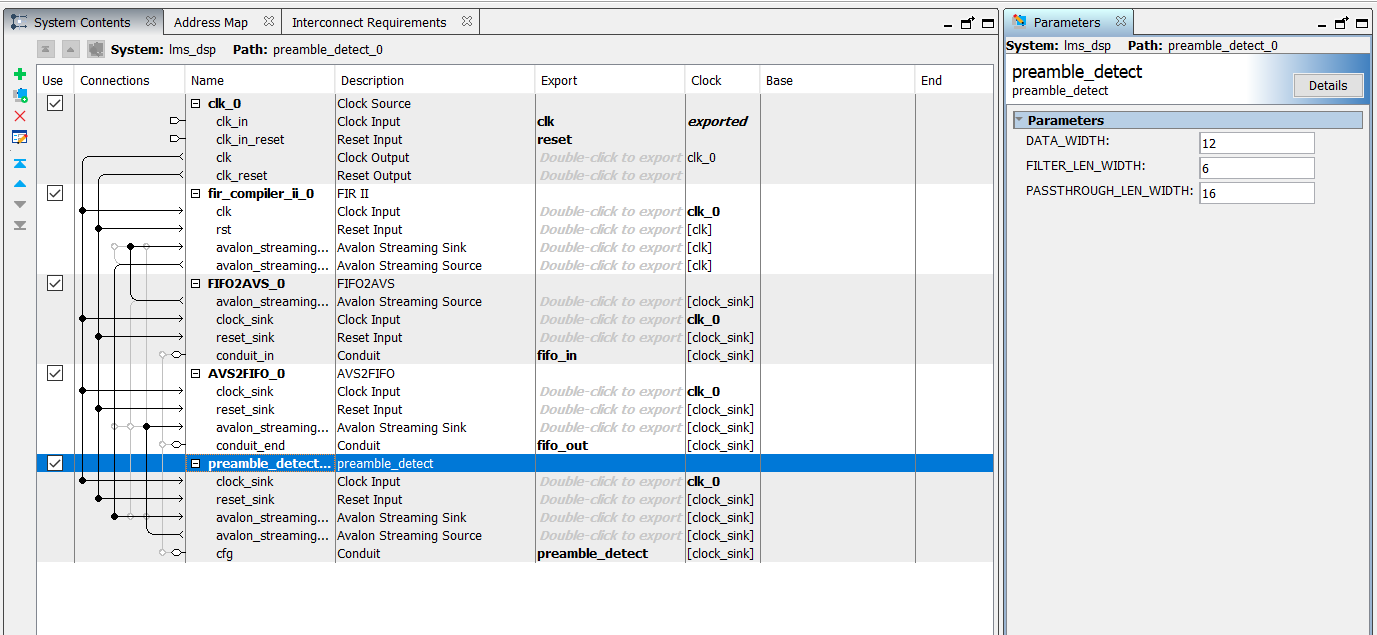
\includegraphics[width=\linewidth]{figures/preamble_detect_qsys_config.PNG}
    \caption{SystemVerilog parameters of the preamble detector in QSYS.}
    \label{fig:pd_hard_param}
\end{figure}

\begin{table}[!h]
\centering
\begin{tabular}{|p{0.36\linewidth}|p{0.48\linewidth}|p{0.08\linewidth}|}
\hline
Parameter & Description & Default value \\
\hline
\textsc{DATA\_WIDTH} & Bit width of the samples & 12 \\
\hline
\textsc{FILTER\_LEN\_WIDTH} & Bit width of the configurable moving average filter length & 6 \\
\hline
\textsc{PASSTHROUGH\_LEN\_WIDTH} & Bit width of the configurable number of samples to pass-through once the threshold is reached & 16 \\
\hline
\end{tabular}
\caption{SystemVerilog parameters of the \texttt{preamble\_detector} IP}
\label{table:pd_hard_param}
\end{table}

\subsection{Configuration signals}
\begin{sloppypar}
Additionally, there are several configuration signals that can be changed during operation from GNU Radio for better flexibility. Those configuration signals are listed in Table \ref{table:pd_soft_param}, you can trace them in the VHDL code, they are coming from the \texttt{fpgacfg} module defined in \texttt{LimeSDR-Mini\_lms7\_lelec210x/src/spi/fpgacfg.vhd}and located in the design hierarchy at \texttt{lms7\_trx\_top/inst0\_nios\_cpu/cfg\_top\_inst1/fpgacfg\_inst0}, as shown in Figure \ref{fig:design_hier_fpgacfg}.
\end{sloppypar}

This module contains a RAM with 16-bit words that retains the configuration of various elements of the FPGA. We used available addresses to put our custom configuration, the address map is written in the repo README. There are default values assigned at reset for the memory bits (Figure \ref{fig:design_hier_fpgacfg}) but they can be changed with a write operation.

\begin{table}[!h]
\centering
\begin{tabular}{|p{0.22\linewidth}|p{0.25\linewidth}|p{0.34\linewidth}|p{0.08\linewidth}|}
\hline
Configuration signal & Description & Allowed values\\
\hline
\texttt{cfg\_enable} & Enable or disable the preamble detector. When disabled, the samples are always passing through. & $\left\{0,1\right\}$ \\
\hline
\texttt{cfg\_FILTER\_LEN} & Size of the moving average filter. & $\left[1,2^{\textsc{FILTER\_LEN\_WIDTH}}-1\right]$ \\
\hline
\texttt{cfg\_PASSTHROUGH\_LEN} & Number of samples to pass-through once the threshold is reached. & $\left[1,2^{\textsc{PASSTHROUGH\_LEN\_WIDTH}}-1\right]$ \\
\hline
\texttt{cfg\_THRESHOLD} & Value to be compared with the moving average filter output. & $\left[1,2^{32}-1\right]$ \\
\hline
\end{tabular}
\caption{Configuration signals \texttt{preamble\_detector} IP}
\label{table:pd_soft_param}
\end{table}

\begin{figure}[!h]
    \centering
    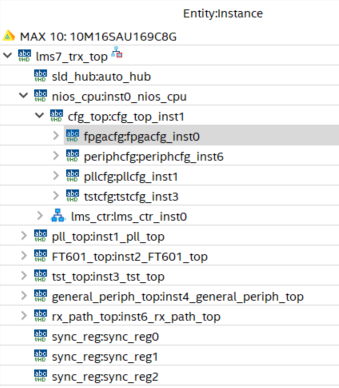
\includegraphics[width=0.3\linewidth]{figures/design_hierarchy_fpgacfg.PNG}
    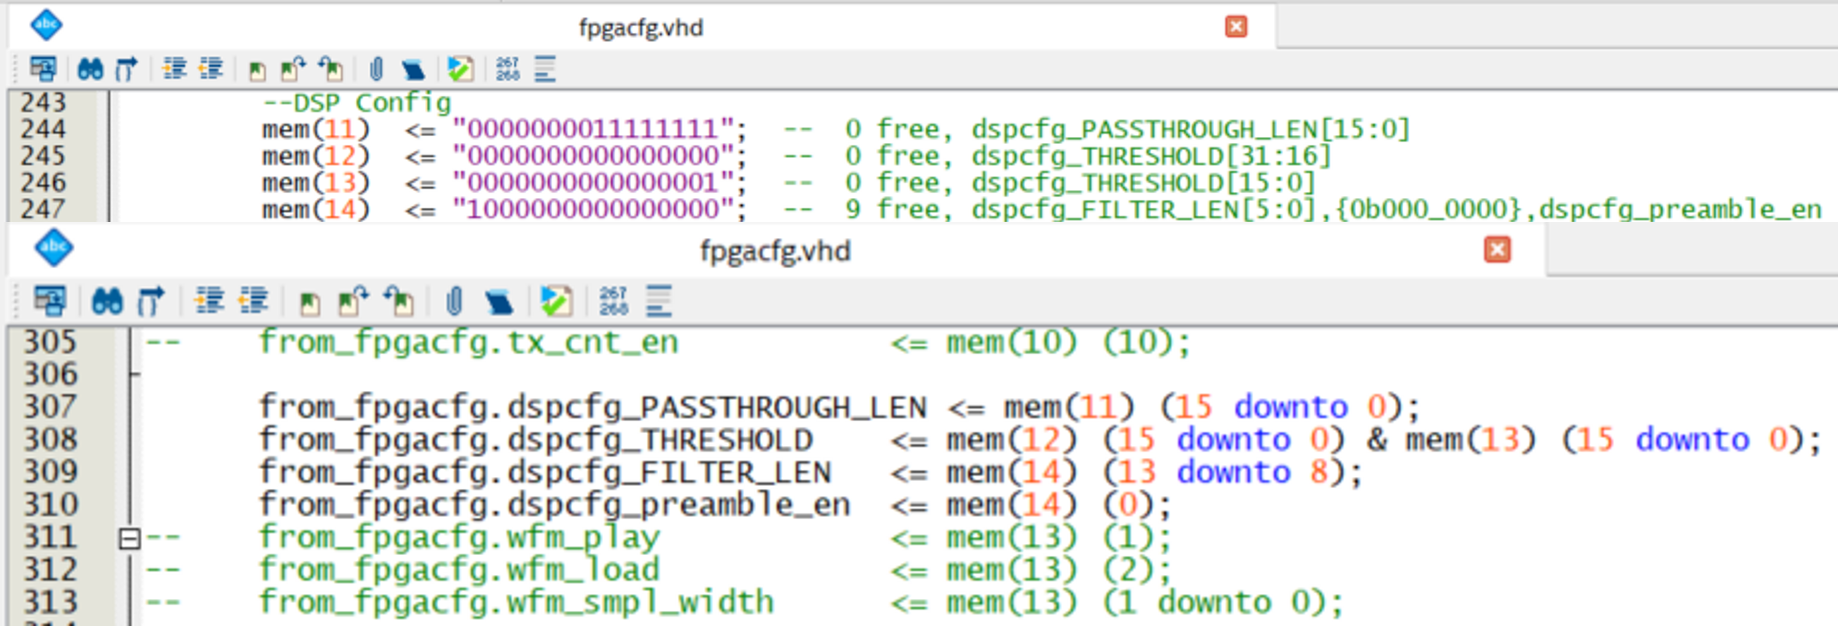
\includegraphics[width=0.6\linewidth]{figures/design_hierarchy_fpgacfg_both.PNG}
    \caption{Configuration signal location in the design hierarchy (left). Assignment and reset values for the DSP configuration signals (right).}
    \label{fig:design_hier_fpgacfg}
\end{figure}

\subsubsection{Read/write operations of the configuration signals from GNU Radio}
The GNU Radio block of the LimeSDR-Mini uses a C++ library called \textit{LimeSuite} in order to write data to the FPGA configuration memory. In the following paragraph, the configuration flow inside LimeSuite and the hardware is briefly described.

\begin{sloppypar}
\paragraph{gr-limesdr GUI interface}
In our custom version of the limeSDR GNU Radio block, we added fields to configure the hardware preamble detector. To do so, we modified the file \texttt{gr-limesdr/grc/limesdr\_fpga\_source.block.yml} and added a GUI callback function named \texttt{set\_dspcfg\_preamble}. This function is in turn defined in \texttt{gr-limesdr/lib/source\_impl.cc} and \texttt{gr-limesdr/lib/device\_handler.cc}. Please take a look at the end of \texttt{device\_handler.cc} and understand the functions we added. At the core of all of them, we use \texttt{modify\_spi\_reg\_bits}, shown in Figure \ref{fig:modify_spi_reg_bits}, that uses LimeSuite \texttt{LMS\_WriteFPGAReg} function. Pay attention to the arguments and try to make the link with the configuration memory of the FPGA, the input structures are defined in \texttt{gr-limesdr/lib/fpga\_register\_map.h}.
\end{sloppypar}

\begin{figure}[!h]
    \centering
    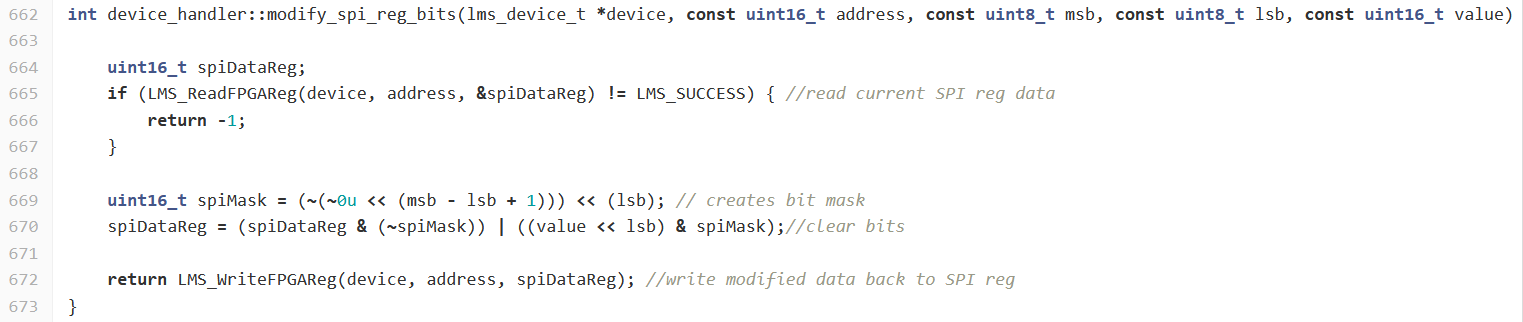
\includegraphics[width=\linewidth]{figures/grlimesdr_write_fpgacfg.PNG}
    \caption{Software interface between GNU Radio and LimeSuite.}
    \label{fig:modify_spi_reg_bits}
\end{figure}

\paragraph{NIOS Interface}
When calling \texttt{LMS\_WriteFPGAReg}, the functions wrap the address and value of the register we wish to configure inside a packet that is transmitted through USB. The complete callstack inside the library is described in the repo README. The USB interface is connected to an FTDI Chip which is in turn interfaced with the FPGA, as shown in Figure \ref{fig:limesdr_mini_schematic}.

Inside the FPGA, we have:
\begin{enumerate}
    \item An FTDI arbitrer that decodes a first part of the packet header to forward it through a configuration FIFO (\texttt{EP02\_fifo}) towards the NIOS subsystem. This arbitration is necessary as we have two other FIFOs coming from the NIOS subsystem and the RX data path (\texttt{EP83\_fifo} and \texttt{EP82\_fifo} respectively).
    \item A NIOS Softcore processor instantiated inside the FPGA reads the FIFO and decodes the second part of the packet header, it then forwards the packet data to through an SPI Master.
    \item An SPI Slave is connected with the configuration memory and writes the received data at the correct address.
\end{enumerate}

\begin{bclogo}[couleur = gray!20, arrondi = 0.2, logo=\bcinfo]{Additional resources}
To help you understand this complex path, we provided you with resources you can find on moodle or \texttt{LimeSDR-Mini\_lms7\_lelec210x/doc/} folder. The file \texttt{FPGA\_config\_path.pdf} with annotations referring to the above paragraph should be helpful, several elements have been hidden to ease the reading. You can also use freely the RTL viewer to skim through the design hierarchy graphically instead of opening files, see Figure \ref{fig:rtl_viewer} for further details.
\end{bclogo}

\begin{figure}[!h]
    \centering
    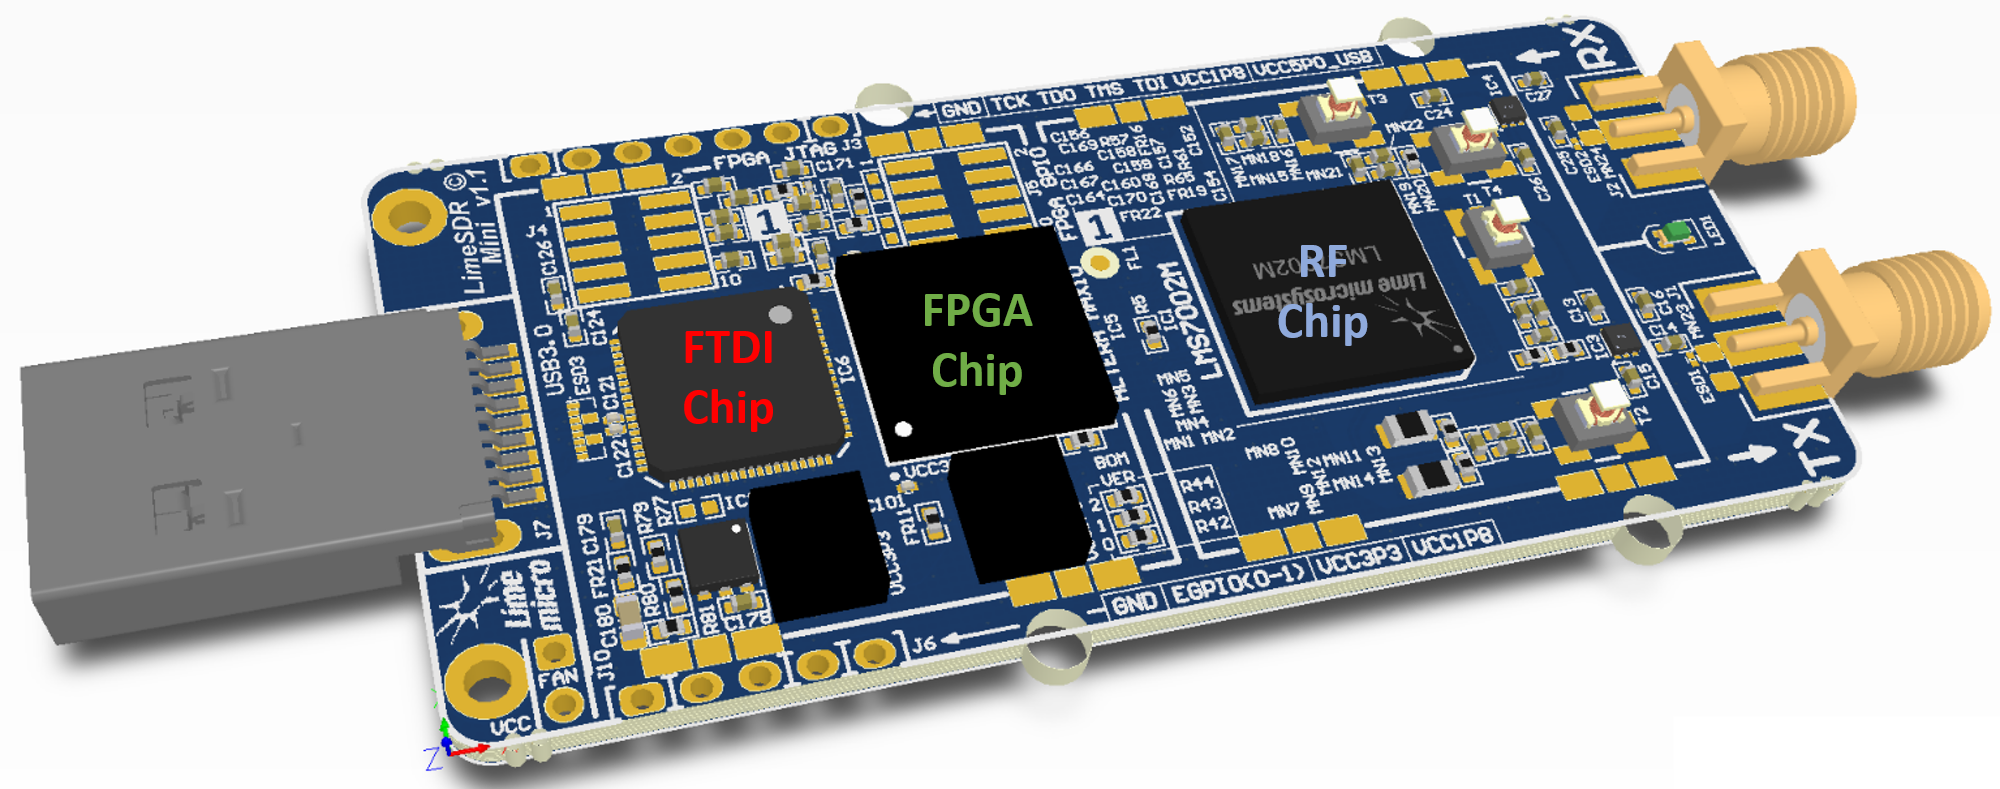
\includegraphics[width=0.7\linewidth]{figures/limesdrmini_schematic.png}
    \caption{Location of the different chips on the LimeSDR-Mini board.}
    \label{fig:limesdr_mini_schematic}
\end{figure}

\begin{figure}[!h]
    \centering
    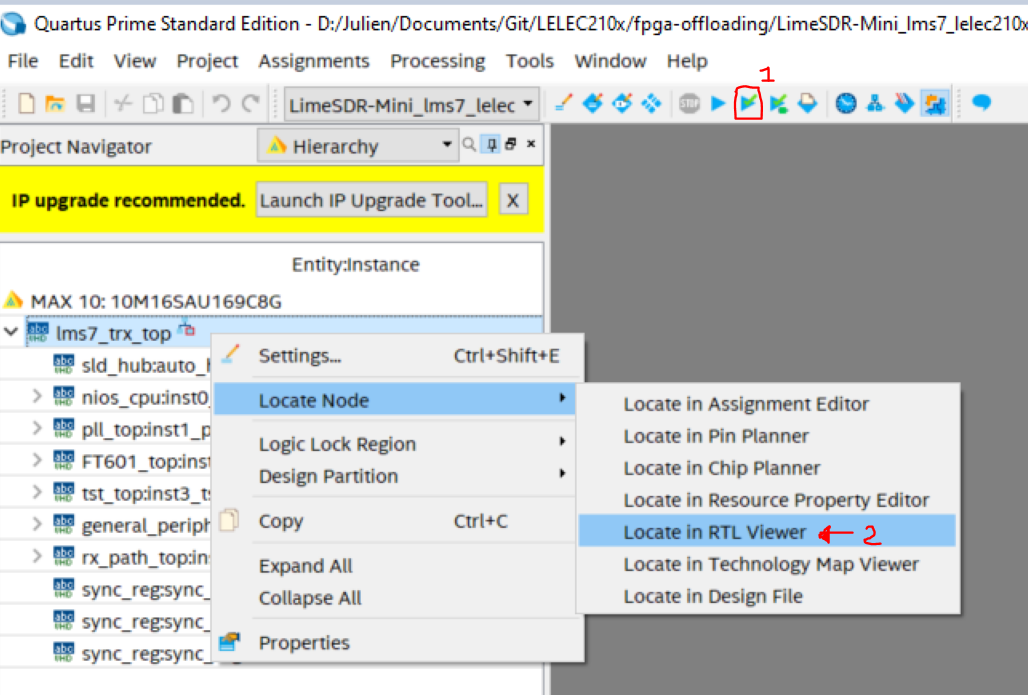
\includegraphics[width=0.7\linewidth]{figures/rtl_viewer.png}
    \caption{In order to use the RTL viewer, first elaborate the design (1) then right click on the design element you want view (2).}
    \label{fig:rtl_viewer}
\end{figure}




\end{document}
%%%%%%%%%%%%%%%%%%%%%%%%%%%%%%%%%%%%%%%%%%%%%%%%%%%%%%%%%%%%%%%%%%%%%%%%%%%%
